\section {NetInf Video Streaming Protocol}\label{VideoDraft}

\subsection{Introduction}

The purpose of this draft is to outline a design and protocol specification for enabling of streaming and chunking data within the current and existing netinf architecture.

\subsubsection{Proposed method of retrieving chunked NDOs}

The stream source will PUBLISH an NDO containing the filename as content. The object is marked as a stream in the metadata. It also contains a locator to the stream source.

In order to access the stream, a receiver will first perform a NetInf-GET on the above filename object in order to retrieve the locator. 

In the next step the client can get the chunks. By replacing the hash algorithm in the NDO-name with \_demo\_ and sending a NetInf-Get to the source, the stream provider will return the octets of the most recent chunk and the chunk number in the metadata. This implies that the regular hash validation has been disabled.

For further chunks, the receiver will increment the chunk number and append it to the locator.
\begin{verbatim}
If a stream is published with the name
 ni:///sha-256;WkOCMB2aEQHrARjTldfhRE5OgZkZmCHzokcoVMnfp2Y

You can get latest chunk by fetching
 ni:///demo;WkOCMB2aEQHrARjTldfhRE5OgZkZmCHzokcoVMnfp2Y

To get first chunk, append a 1 to the end of the hash
 ni:///demo;WkOCMB2aEQHrARjTldfhRE5OgZkZmCHzokcoVMnfp2Y1

To get the 32th chunk, append 32 to the end of the hash
 ni:///demo;WkOCMB2aEQHrARjTldfhRE5OgZkZmCHzokcoVMnfp2Y32
\end{verbatim}
 
If the receiver also acts as a cache, it will send a PUBLISH with the filename object and a locator pointing to itself to the NRS.
\fig{streaming_dia} shows the flow of the actions. 
\\

\begin{figure}
\centering
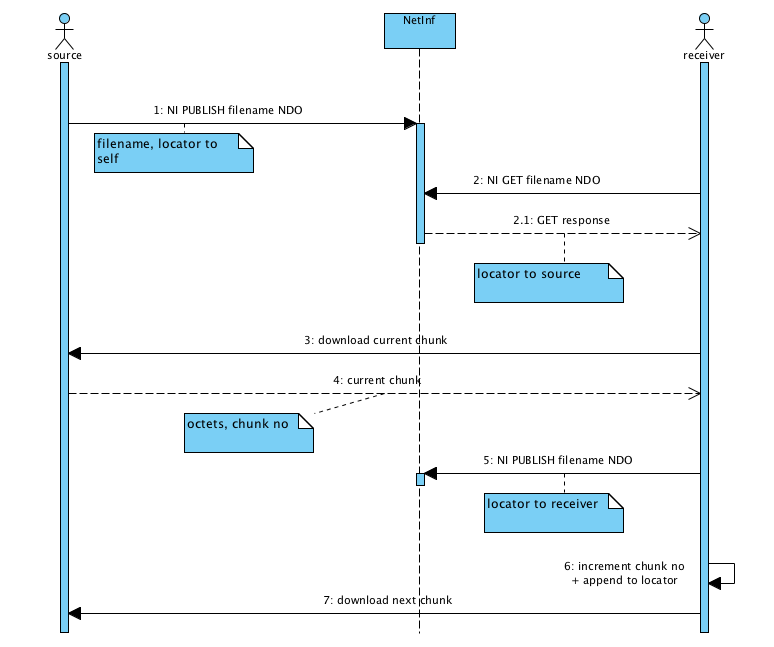
\includegraphics[scale=0.5]{./img/sequence_diagram_streaming.png}
\caption{Streaming Sequence Diagram}\label{fig:streaming_dia}
\end{figure}


\subsubsection{Testing criteria} 

For a simple test setup, in addition to the NetInf node, a receiving and a publishing client is required. A more sophisticated test could involve multiple receivers, to demonstrate the caching.

A use case for testing is one where the source of the content is a pre-encoded video file of a particular size.

The example below assumes a video file of the size 700 megabytes.

A client (Publisher) will have a default chunk size which is used to chunk up the source file. For this example, 1 megabyte chunks will be used.

Thus, it can be calculated that the publisher will create 700 chunks of the size 1 megabyte, numbered 1-700.

A second client (receiver) knowing the name of the video file will then send a Get request to the NetInf node (to keep things simple, it is assumed that the object's name is already known).

The client will now start generating consecutive GET requests with the sequence numbers constantly increasing and expect to receive the appropriate chunk.

As well as  poll the NRS for new locators, to get better load balance between nodes contributing to the stream.

This process occures until the GET requests generate a 404 because the unique sequence number has increased past the last published chunk number.

\subsubsection{Extra notes}

Chunk size is going to be a configurable option in the publishing client.
